\documentclass[a4paper,12pt]{article}
\usepackage[utf8]{inputenc}

\usepackage[catalan]{babel}
\usepackage{fancyhdr} % Per la capçalera
\usepackage{geometry}
\usepackage{graphicx} % Per importar logos (i altres gràfics)
\usepackage[colorlinks,linkcolor=black]{hyperref} % Per fer que l'index tingui hiperlinks en el pdf
\usepackage{parskip}
\usepackage[sc,small]{titlesec} % Seccions personalitzades

%% Títols
\newcommand{\modulnum}{5}
\newcommand{\modulnom}{Entorns de Desenvolupament}

\newcommand{\ufnum}{1}
\newcommand{\ufnom}{Desenvolupament de Programari}

\newcommand{\acttipus}{Pràctica 1.2}
\newcommand{\actnom}{Projecte SummerField}

%% Entreliniats
\linespread{1.5}

%% Capçalera
\pagestyle{fancy}
\setlength{\headheight}{40pt}
\addtolength{\topmargin}{-20pt}
\fancyhead[L]{\includegraphics*[height=\headheight]{provencana_bw.pdf}}
\fancyhead[R]{
	{\scshape\scriptsize Mòdul \modulnum: \modulnom}\\
	{\scshape\footnotesize \acttipus \space - \actnom}\\
	{\scshape\small Eina Coma Bages i Iris Hidalgo Palomino}}

\addtolength{\textheight}{2cm}

%% Comandes personalitzades
\newcommand{\mygraphic}[2][width=0.9\textwidth]{\begin{center}
		\centering\includegraphics[#1]{#2}\par
\end{center}}

\renewcommand{\contentsname}{Índex}

\begin{document}
\begin{titlepage}
	\centering
	\includegraphics*[width=0.15\textwidth]{provencana_color.pdf}
	\par\vspace{0.5cm}

	{\scshape\Large Institut Provençana \par}

	\vspace{1cm}

	{\itshape\Large \acttipus \par}
	{\bfseries\LARGE \actnom \par}
	
	\vspace{1cm}
	
	{\scshape\large Mòdul \modulnum: \par}
	{\scshape\Large \modulnom \par}

	\vspace{1cm}
	
	{\scshape\normalsize Unitat Formativa \ufnum: \par}
	{\scshape\large \ufnom \par}

	\vfill
	{\Large\itshape \autor \par}
	\vfill

	Curs 2022/2023
\end{titlepage}
\tableofcontents
\newpage

\section{Tasca 1}
\subsection{Requisits Funcionals}

\begin{description}
	\item[S01 Disponibilitat producte:] Com a dependent vull consultar la disponibilitat d'un producte, per poder informar un client que el demani.
	\item[S02 Factura i ingrés:] Com a dependent vull poder crear una factura i ingressar els diners, per tenir el registre de les compres.
	\item[S03 Actualització inventari:] Com a dependent vull que quan es faci una venda es descompti de l'inventari, per tenir l'inventari actualitzat.
\end{description}


\begin{description}
	\item[S04 Encarregat Magatzem i Dependent:] Com a encarregat d'un magatzem de botiga vull poder gestionar l'estat del magatzem i també atendre a clients, per desenvolupar la meva feina.
	\item[S05 Comanda magatzem:] Com a encarregat d'un magatzem de botiga vull poder mirar si hi ha un producte baix en stock per demanar-lo al magatzem.
\end{description}

\begin{description}
	\item[S06 Gestió personal botiga:] Com a encarregat d'una botiga vull poder donar d'alta o de baixa a qualsevol dependent per gestionar la contractació.
    \item[S07 Alta producte botiga:] Com a encarregat d'una botiga vull poder donar d'alta un producte, per poder-lo introduir a la botiga.
    \item[S08 Encarregat Botiga i Dependent:] Com a encarregat d'una botiga vull poder fer les tasques de dependent.
\end{description}

\begin{description}
	\item[S09 Recepció comandes:] Com a responsable de magatzem vull poder rebre les peticions de material de botigues i altres magatzems per poder atendre-les.
	\item[S11 Provisió botiga:] Com a responsable de magatzem vull poder subministrar les comandes a les botigues de manera immediata perquè no es quedin sense stock.
	\item[S12 Provisió altres magatzem:] Com a responsable de magatzem vull subministrar les comandes als magatzems només si això no implica quedar-me amb menys de la meitat del que he definit com a "baix de stock", per no quedar-me sense stock servint a un altre magatzem.
	\item[S13 Revisió inventari:] Com a responsable de magatzem vull revisar l'inventari un cop al dia per demanar els que estan marcats com a baix d'stock, per no quedar-me sense inventari.
	\item[S14 Provisió stock:] Com a responsable de magatzem vull que el sistema demani a altres magatzems o a proveïdors els ítems baixos en stock, per no quedar-me sense stock.
	\item[S15 Gestió personal magatzem:] Com a responsable de magatzem vull poder contractar i donar de baixa, per gestionar la contractació.
\end{description}

\begin{description}
	\item[S16 Alta productes nous:] Com a director comercial vull poder donar d'alta els productes a la base de dades general, perquè estiguin disponibles a les botigues.
	\item[S17 Configuració marges de benefici:] Com a director comercial
	vull poder definir els marges de beneficis de les categories per a definir els preus.
\end{description}

\subsection{Requisits No Funcionals}
\textbf{Requisits de desenvolupament:} La programació es farà en Java i el SGBD serà MySQL o PostgreSQL

\textbf{Requisits de seguretat:} Hem de tenir un control dels usuaris i de a quines funcions poden accedir (l'encarregat de botiga ha de poder gestionar la contractació però el dependent no).

\textbf{Requisits de fiabilitat:} L'aplicatiu de botigues ha de funcionar com a mínim mentre les botigues estiguin obertes.

\textbf{Requisits regulatius:} Les dades de personal s'han d'emmagatzemar d'acord amb la legislació de protecció de dades.

\textbf{Requisits de compatibilitat:} El programa ha de ser compatible amb els terminals ja existents a botigues i magatzems.

\section{Tasca 2}
\subsection{Product Backlog}
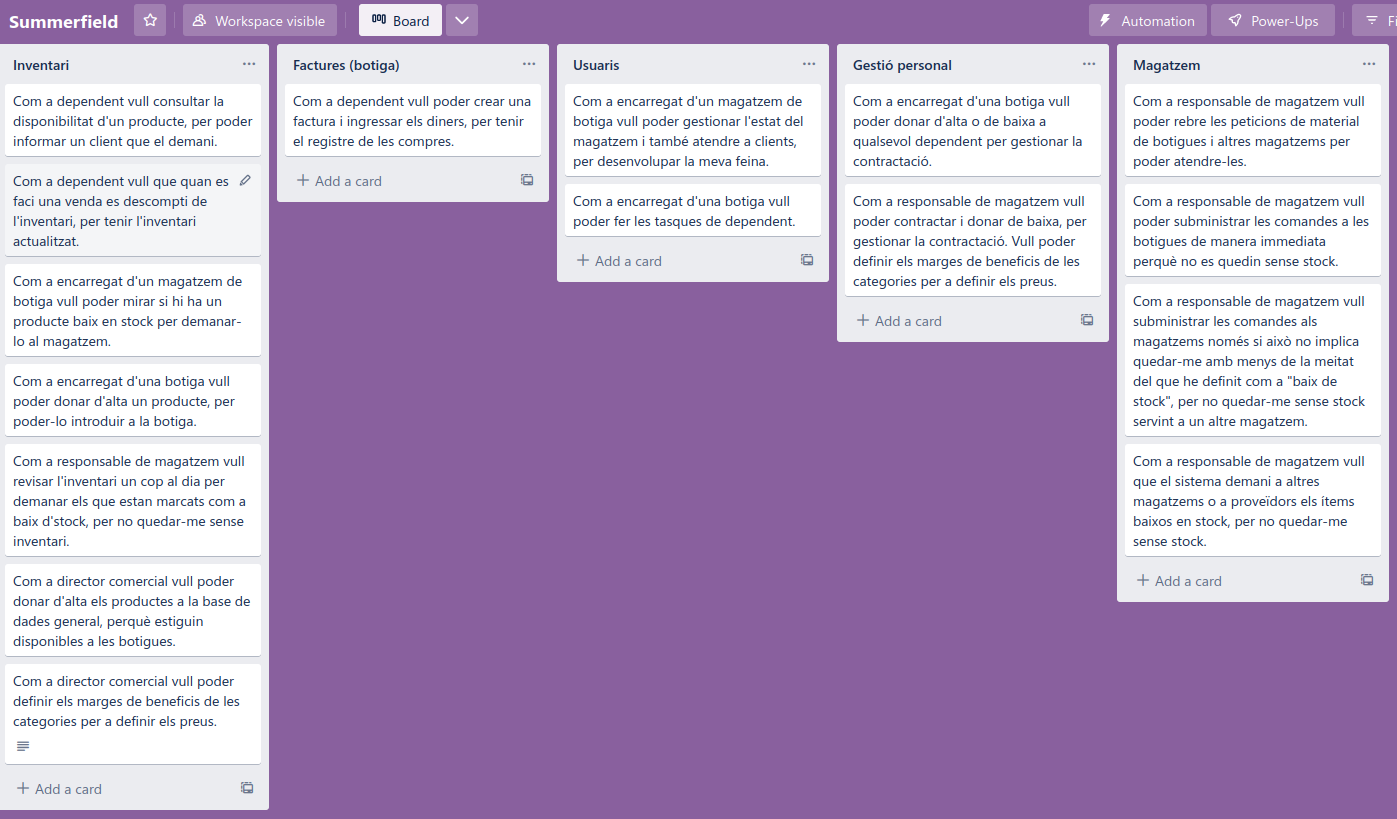
\includegraphics[width=\textwidth]{imatges/stories_trello.png}

\subsection{Puntuació i priorització}

\begin{enumerate}
	\item\textbf{Puntuació:} \textit{3} \textbf{S07 Alta producte botiga:} Com a encarregat d'una botiga vull poder donar d'alta un producte, per poder-lo introduir a la botiga.

	\item\textbf{Puntuació:} \textit{4} \textbf{S16 Alta productes nous:} Com a director comercial vull poder donar d'alta els productes a la base de dades general, perquè estiguin disponibles a les botigues.
	
	\item\textbf{Puntuació:} \textit{3} \textbf{S17 Configuració marges de benefici:} Com a director comercial vull poder definir els marges de beneficis de les categories per a definir els preus.
	
	\item\textbf{Puntuació:} \textit{5} \textbf{S01 Disponibilitat producte:} Com a dependent vull consultar la disponibilitat d'un producte, per poder informar un client que el demani.
	
	\item\textbf{Puntuació:} \textit{6} \textbf{S03 Actualització inventari:} Com a dependent vull que quan es faci una venda es descompti de l'inventari, per tenir l'inventari actualitzat.
	
	\item\textbf{Puntuació:} \textit{6} \textbf{S13 Revisió inventari:} Com a responsable de magatzem vull revisar l'inventari un cop al dia per demanar els que estan marcats com a baix d'stock, per no quedar-me sense inventari.
	
	\item\textbf{Puntuació:} \textit{5} \textbf{S05 Comanda magatzem:} Com a encarregat d'un magatzem de botiga vull poder mirar si hi ha un producte baix en stock per demanar-lo al magatzem.
	
	\item\textbf{Puntuació:} \textit{4} \textbf{S09 Recepció comandes:} Com a responsable de magatzem vull poder rebre les peticions de material de botigues i altres magatzems per poder atendre-les.
	
	\item\textbf{Puntuació:} \textit{8} \textbf{S11 Provisió botiga:} Com a responsable de magatzem vull poder subministrar les comandes a les botigues de manera immediata perquè no es quedin sense stock.
	
	\item\textbf{Puntuació:} \textit{9} \textbf{S12 Provisió altres magatzem:} Com a responsable de magatzem vull subministrar les comandes als magatzems només si això no implica quedar-me amb menys de la meitat del que he definit com a "baix de stock", per no quedar-me sense stock servint a un altre magatzem.
	
	\item\textbf{Puntuació:} \textit{7} \textbf{S14 Provisió stock:} Com a responsable de magatzem vull que el sistema demani a altres magatzems o a proveïdors els ítems baixos en stock, per no quedar-me sense stock.
	
	\item\textbf{Puntuació:} \textit{3} \textbf{S04 Encarregat Magatzem i Dependent:} Com a encarregat d'un magatzem de botiga vull poder gestionar l'estat del magatzem i també atendre a clients, per desenvolupar la meva feina.
	
	\item\textbf{Puntuació:} \textit{3} \textbf{S08 Encarregat Botiga i Dependent:} Com a encarregat d'una botiga vull poder fer les tasques de dependent.
	
	\item\textbf{Puntuació:} \textit{6} \textbf{S06 Gestió personal botiga:} Com a encarregat d'una botiga vull poder donar d'alta o de baixa a qualsevol dependent per gestionar la contractació.
	
	\item\textbf{Puntuació:} \textit{6} \textbf{S15 Gestió personal magatzem:} Com a responsable de magatzem vull poder contractar i donar de baixa, per gestionar la contractació. Vull poder definir els marges de beneficis de les categories per a definir els preus.
	
	\item\textbf{Puntuació:} \textit{2} \textbf{S02 Factura i ingrés:} Com a dependent vull poder crear una factura i ingressar els diners, per tenir el registre de les compres.
\end{enumerate}

\section{Tasca 3}
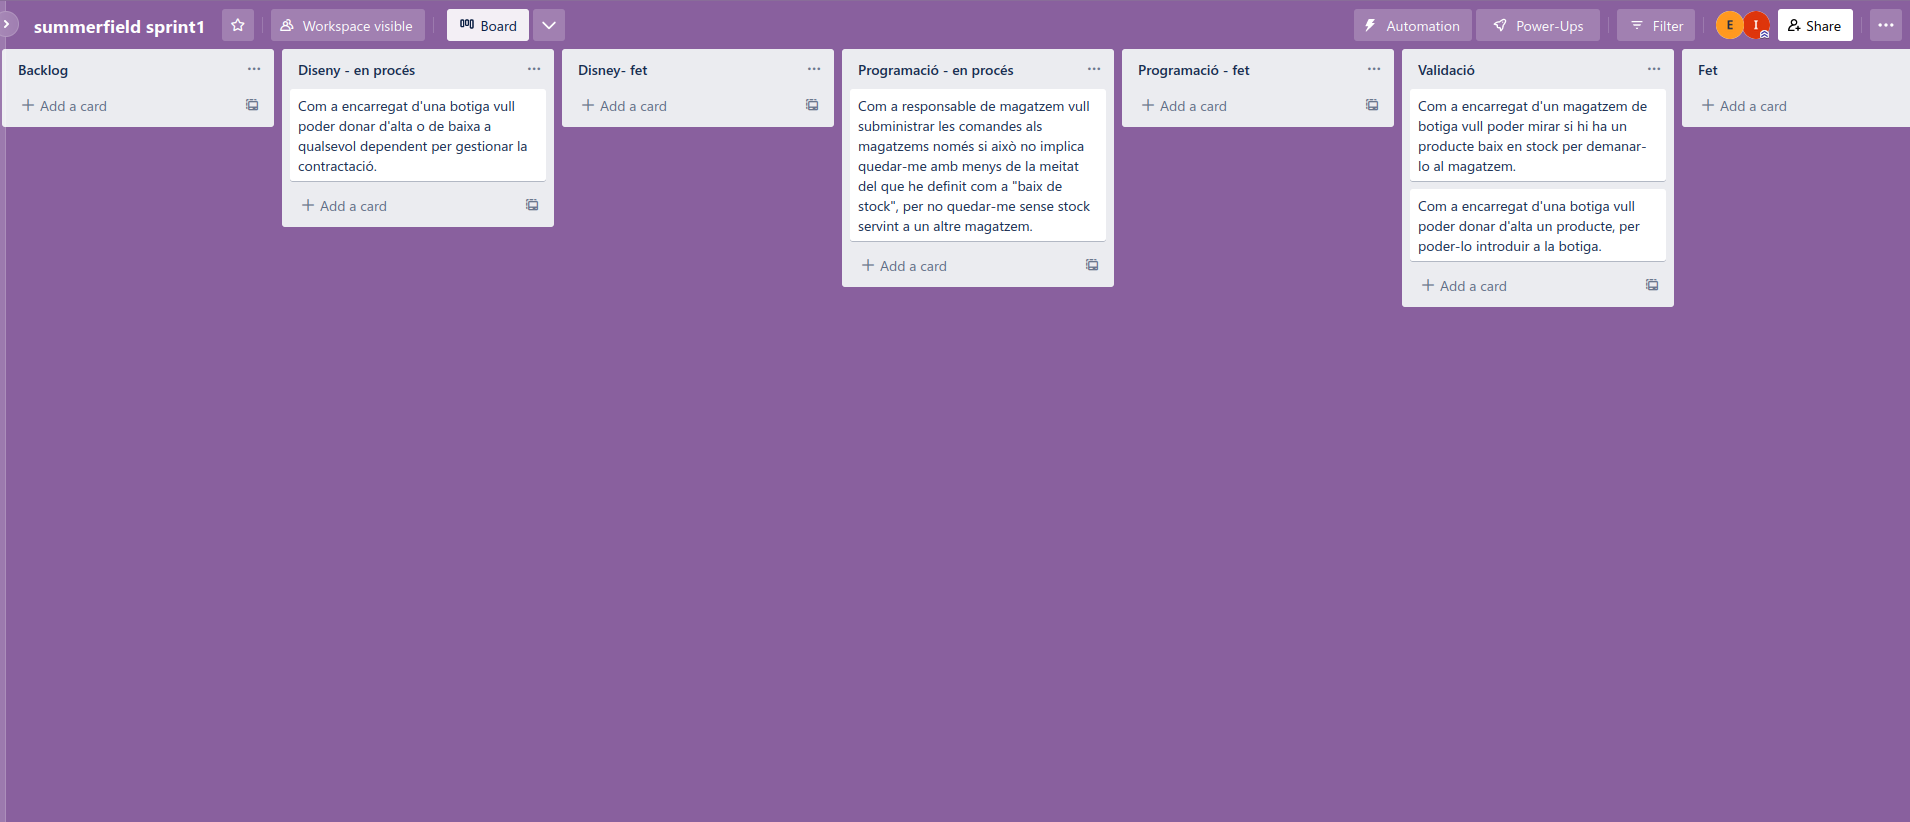
\includegraphics[width=\textwidth]{imatges/trello_sprint1.png}
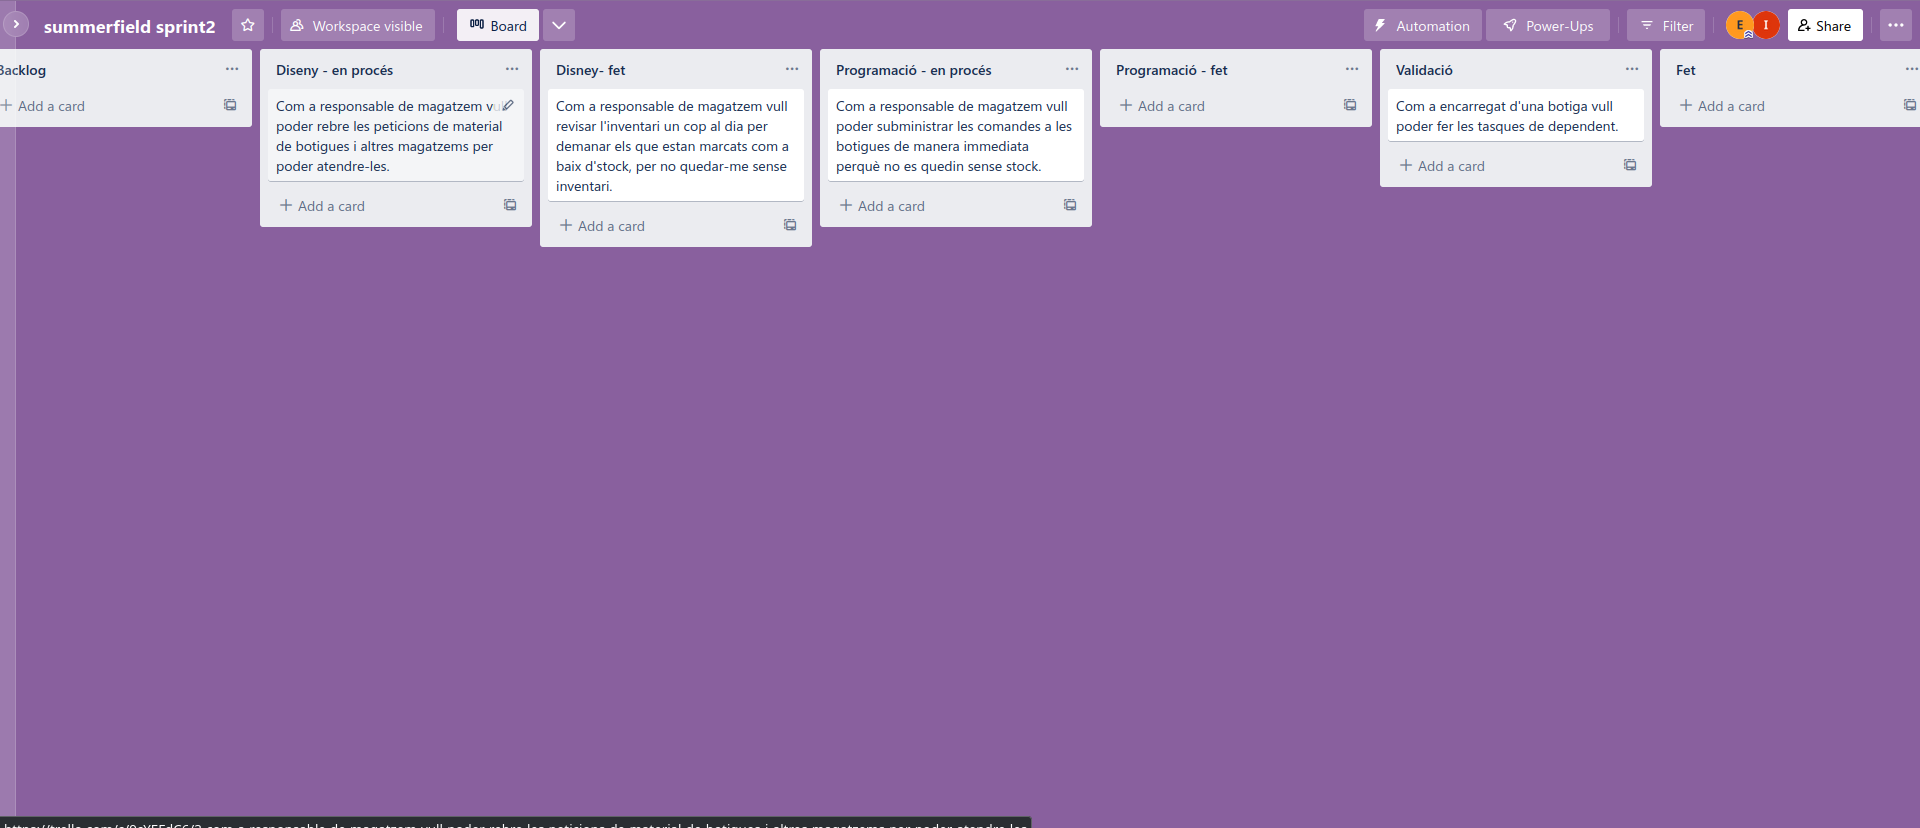
\includegraphics[width=\textwidth]{imatges/trello_sprint2.png}
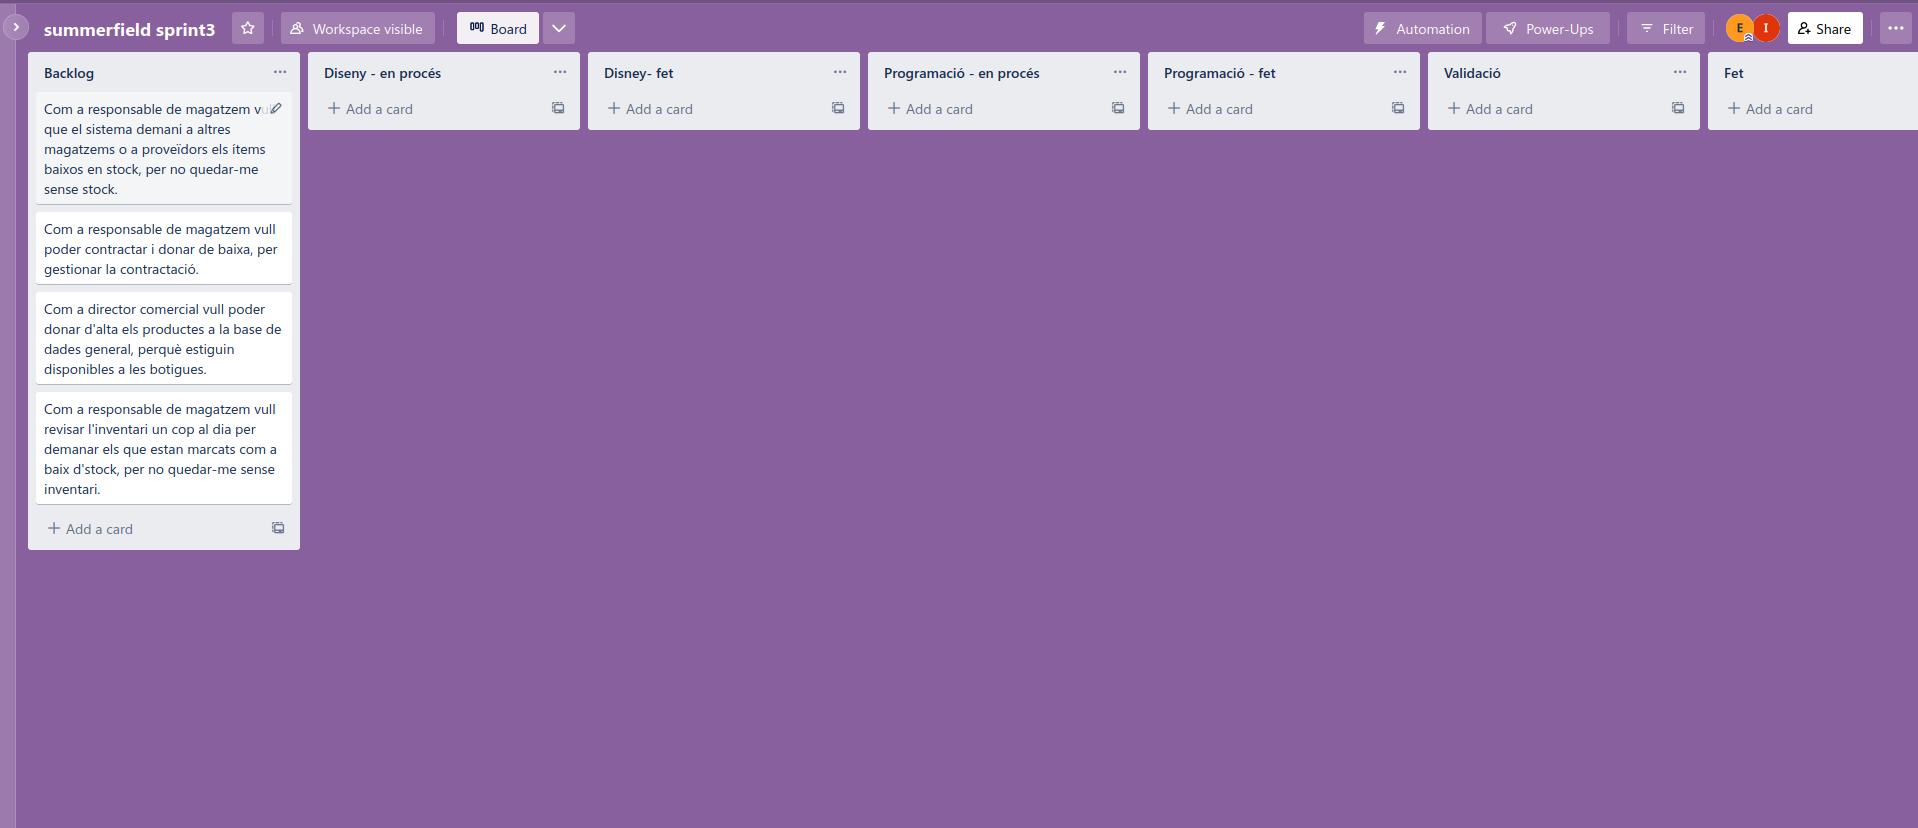
\includegraphics[width=\textwidth]{imatges/trello_sprint3.png}
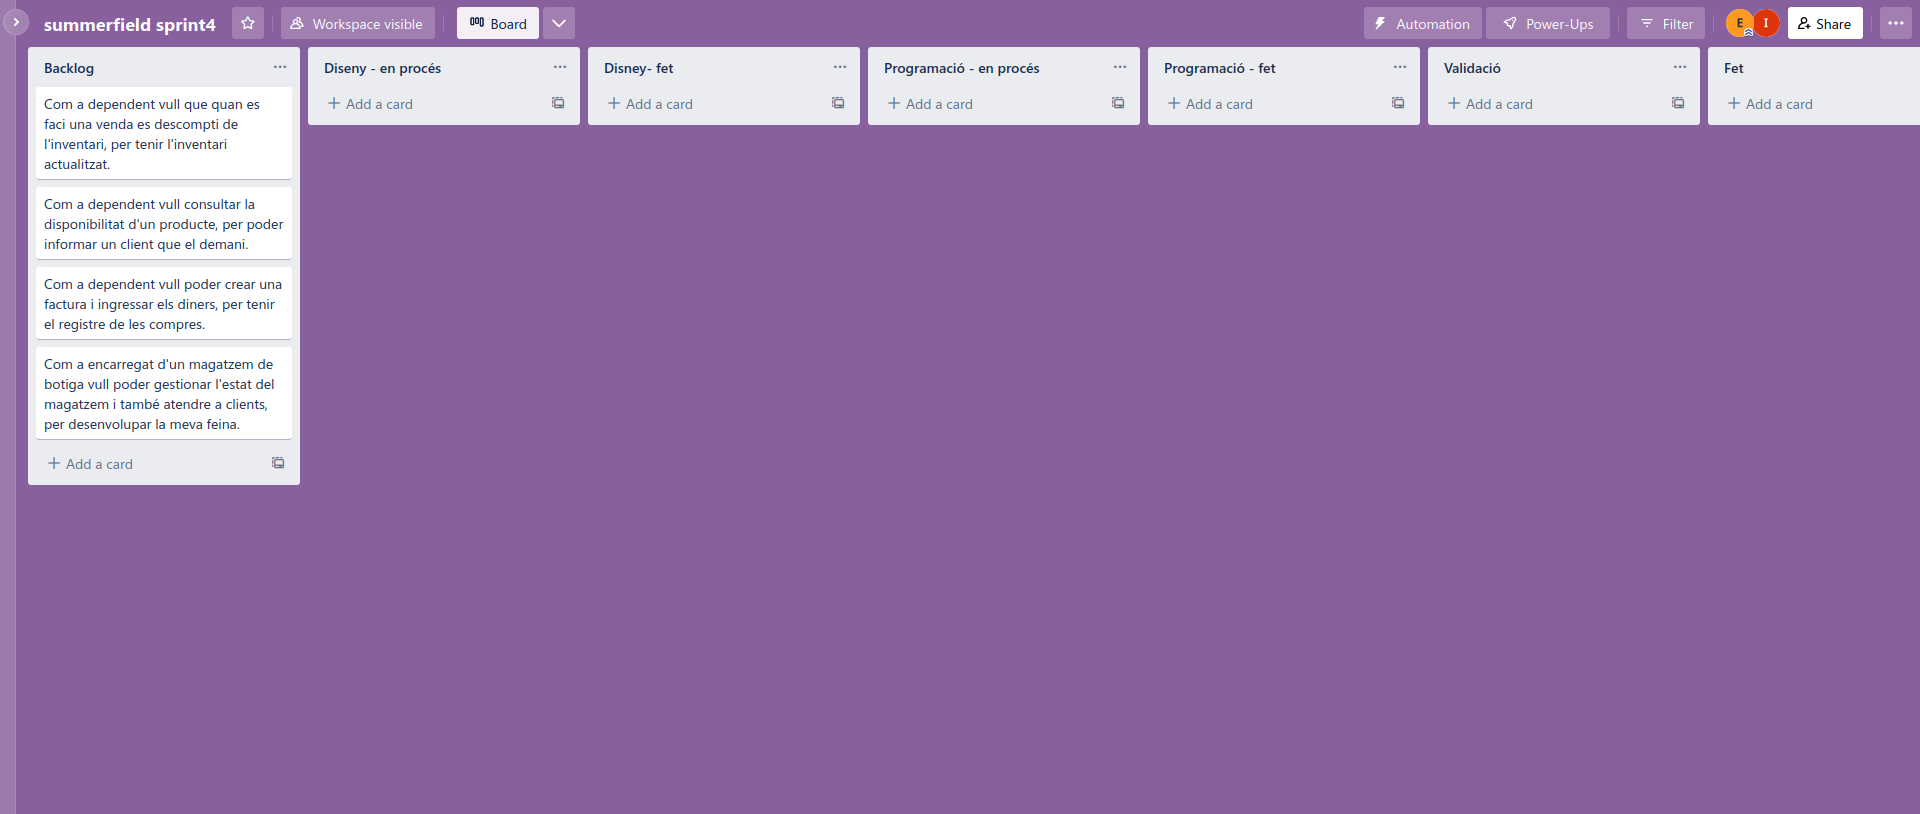
\includegraphics[width=\textwidth]{imatges/trello_sprint4.png}
\end{document}